\documentclass[12pt]{article}

\usepackage{amsmath, amssymb}
\usepackage[margin=1in]{geometry}
\usepackage{helvet}
\renewcommand{\familydefault}{\sfdefault}
\def\newrule#1#2#3{\begin{center}
    {#1} \\
    \line(1,0){300} {}{}{}{}{}{}{} [{#3}]\\
    {#2}
\end{center}}

\begin{document}
\def\assignment{Homework 04}

\pagenumbering{gobble}
\noindent{\large COSC 4200 \hfill Name: \underline{Jacob Tuttle} \\ Computability and Complexity}
\begin{center}
    {\Large \assignment} \\ \textbf{\today}
\end{center}


\begin{enumerate}
    \item\begin{enumerate}
        \item Perform a product construction of $A$ and $B$ where the only accepting states are ones in which both $A$ and $B$ accept. Then, perform a product construction of that new DFA with $C$. Accepting states are states in which $A \cap B$ or $C$ are accepting. The DFA will have $n_an_bn_c$ states.

        \item Perform a product construction on $A$ and $B$. The accepting states will be all states where either $A$ or $B$ accepts. Then perform a cline closure by taking the union of all possible $(A \cup B)^k$ for all $k \leq \infty$. This effectively tacks on every possible combination of strings in $A \cup B$ into the closure. There are an indeterminate amount of states.

        \item Perform a concatination of $A$ and $B$ by establishing free moves from accepting states in $A$ to the first state in $B$. Convert that NFA to a DFA. Then, use product construction on the resulting DFA with $C$ where accepting states are ones in which $A \cdot B$ and $C$ are in accepting states. The DFA will have $(n_a + n_b) * n_c$ states.

        \item Perform a cline closure as described in part (b) on $A$. Then perform a product construction on the resulting $A*$ and $B$. Accepting states are all states in which both $A*$ and $B$ are accepting. Then take all states that aren't accepting states and make them accept while taking all previously accepting states and making them reject to complete the complement. Finally, perform the concatination operation as described in (c) on the new DFA and $C$.
    \end{enumerate}
    \item\begin{enumerate}
        \item This DFA can be formed by taking the union of two DFAs: one that fails if the substring 101 is present (top) and one that succeeds when the length of x is a multiple of 3 (bottom).
        \begin{center}
        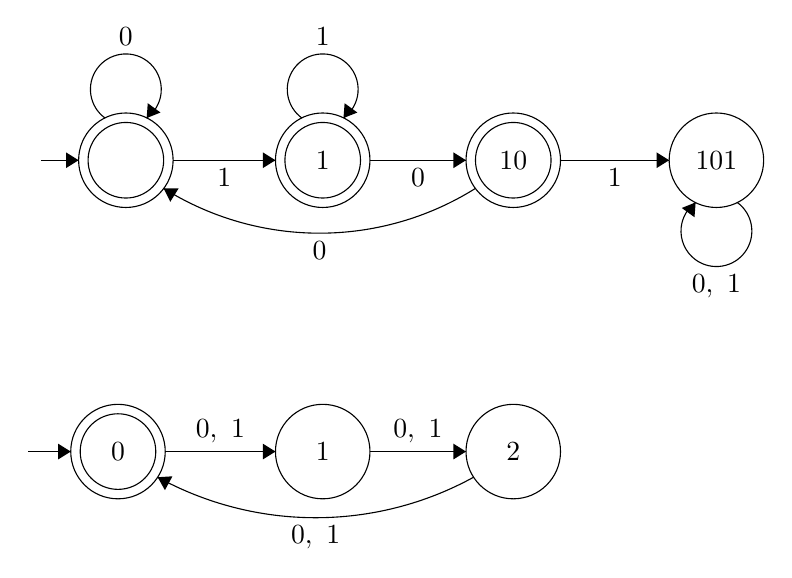
\begin{tikzpicture}[scale=0.2]
        \tikzstyle{every node}+=[inner sep=0pt]
        \draw [black] (8.8,-11) circle (3);
        \draw [black] (8.8,-11) circle (2.4);
        \draw [black] (21.3,-11) circle (3);
        \draw (21.3,-11) node {$1$};
        \draw [black] (21.3,-11) circle (2.4);
        \draw [black] (33.4,-11) circle (3);
        \draw (33.4,-11) node {$10$};
        \draw [black] (33.4,-11) circle (2.4);
        \draw [black] (46.3,-11) circle (3);
        \draw (46.3,-11) node {$101$};
        \draw [black] (8.3,-29.5) circle (3);
        \draw (8.3,-29.5) node {$0$};
        \draw [black] (8.3,-29.5) circle (2.4);
        \draw [black] (21.3,-29.5) circle (3);
        \draw (21.3,-29.5) node {$1$};
        \draw [black] (33.4,-29.5) circle (3);
        \draw (33.4,-29.5) node {$2$};
        \draw [black] (3.4,-11) -- (5.8,-11);
        \fill [black] (5.8,-11) -- (5,-10.5) -- (5,-11.5);
        \draw [black] (7.477,-8.32) arc (234:-54:2.25);
        \draw (8.8,-3.75) node [above] {$0$};
        \fill [black] (10.12,-8.32) -- (11,-7.97) -- (10.19,-7.38);
        \draw [black] (47.623,-13.68) arc (54:-234:2.25);
        \draw (46.3,-18.25) node [below] {$0,\mbox{ }1$};
        \fill [black] (44.98,-13.68) -- (44.1,-14.03) -- (44.91,-14.62);
        \draw [black] (36.4,-11) -- (43.3,-11);
        \fill [black] (43.3,-11) -- (42.5,-10.5) -- (42.5,-11.5);
        \draw (39.85,-11.5) node [below] {$1$};
        \draw [black] (24.3,-11) -- (30.4,-11);
        \fill [black] (30.4,-11) -- (29.6,-10.5) -- (29.6,-11.5);
        \draw (27.35,-11.5) node [below] {$0$};
        \draw [black] (11.8,-11) -- (18.3,-11);
        \fill [black] (18.3,-11) -- (17.5,-10.5) -- (17.5,-11.5);
        \draw (15.05,-11.5) node [below] {$1$};
        \draw [black] (19.977,-8.32) arc (234:-54:2.25);
        \draw (21.3,-3.75) node [above] {$1$};
        \fill [black] (22.62,-8.32) -- (23.5,-7.97) -- (22.69,-7.38);
        \draw [black] (30.996,-12.79) arc (-57.94353:-122.05647:18.646);
        \fill [black] (11.2,-12.79) -- (11.62,-13.64) -- (12.15,-12.79);
        \draw (21.1,-16.13) node [below] {$0$};
        \draw [black] (2.6,-29.5) -- (5.3,-29.5);
        \fill [black] (5.3,-29.5) -- (4.5,-29) -- (4.5,-30);
        \draw [black] (11.3,-29.5) -- (18.3,-29.5);
        \fill [black] (18.3,-29.5) -- (17.5,-29) -- (17.5,-30);
        \draw (14.8,-29) node [above] {$0,\mbox{ }1$};
        \draw [black] (24.3,-29.5) -- (30.4,-29.5);
        \fill [black] (30.4,-29.5) -- (29.6,-29) -- (29.6,-30);
        \draw (27.35,-29) node [above] {$0,\mbox{ }1$};
        \draw [black] (30.883,-31.128) arc (-61.23349:-118.76651:20.848);
        \fill [black] (10.82,-31.13) -- (11.28,-31.95) -- (11.76,-31.07);
        \draw (20.85,-34.2) node [below] {$0,\mbox{ }1$};
        \end{tikzpicture}
        \end{center}

        \item This DFA is most easily represented by the intersection of two sub-DFAs, presented below. One counts the difference between the number of 0s and the number of 1s (top) and one counts the binary value of x mod 3 (bottom).
        \begin{center}
        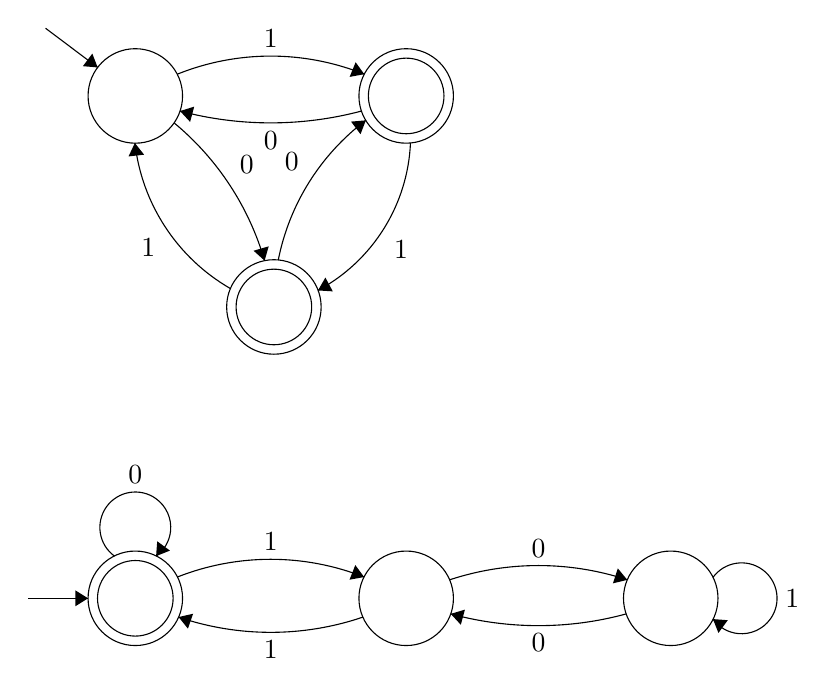
\begin{tikzpicture}[scale=0.2]
        \tikzstyle{every node}+=[inner sep=0pt]
        \draw [black] (8.6,-8.6) circle (3);
        \draw [black] (25.8,-8.6) circle (3);
        \draw [black] (25.8,-8.6) circle (2.4);
        \draw [black] (17.4,-22) circle (3);
        \draw [black] (17.4,-22) circle (2.4);
        \draw [black] (8.6,-40.5) circle (3);
        \draw [black] (8.6,-40.5) circle (2.4);
        \draw [black] (25.8,-40.5) circle (3);
        \draw [black] (42.6,-40.5) circle (3);
        \draw [black] (11.26,-7.222) arc (111.97447:68.02553:15.875);
        \fill [black] (23.14,-7.22) -- (22.59,-6.46) -- (22.21,-7.39);
        \draw (17.2,-5.57) node [above] {$1$};
        \draw [black] (26.073,-11.579) arc (-2.45257:-61.7118:11.183);
        \fill [black] (20.2,-20.95) -- (21.14,-21.01) -- (20.67,-20.13);
        \draw (25,-18.33) node [right] {$1$};
        \draw [black] (14.644,-20.834) arc (-119.93285:-173.48002:12.272);
        \fill [black] (8.57,-11.59) -- (8.17,-12.44) -- (9.16,-12.33);
        \draw (9.9,-18.26) node [left] {$1$};
        \draw [black] (22.96,-9.56) arc (-75.1464:-104.8536:22.47);
        \fill [black] (11.44,-9.56) -- (12.08,-10.25) -- (12.34,-9.28);
        \draw (17.2,-10.81) node [below] {$0$};
        \draw [black] (17.678,-19.018) arc (-191.18849:-232.97588:14.674);
        \fill [black] (23.24,-10.15) -- (22.3,-10.23) -- (22.9,-11.03);
        \draw (19.01,-12.78) node [left] {$0$};
        \draw [black] (11.061,-10.309) arc (50.40094:16.18619:17.8);
        \fill [black] (16.81,-19.06) -- (17.07,-18.15) -- (16.11,-18.43);
        \draw (15.21,-12.93) node [right] {$0$};
        \draw [black] (2.9,-4.3) -- (6.21,-6.79);
        \fill [black] (6.21,-6.79) -- (5.87,-5.91) -- (5.27,-6.71);
        \draw [black] (1.8,-40.5) -- (5.6,-40.5);
        \fill [black] (5.6,-40.5) -- (4.8,-40) -- (4.8,-41);
        \draw [black] (11.273,-39.148) arc (111.50828:68.49172:16.165);
        \fill [black] (23.13,-39.15) -- (22.57,-38.39) -- (22.2,-39.32);
        \draw (17.2,-37.52) node [above] {$1$};
        \draw [black] (23.052,-41.695) arc (-71.22923:-108.77077:18.186);
        \fill [black] (11.35,-41.69) -- (11.94,-42.43) -- (12.27,-41.48);
        \draw (17.2,-43.16) node [below] {$1$};
        \draw [black] (28.557,-39.327) arc (108.27118:71.72882:17.998);
        \fill [black] (39.84,-39.33) -- (39.24,-38.6) -- (38.93,-39.55);
        \draw (34.2,-37.92) node [above] {$0$};
        \draw [black] (39.771,-41.491) arc (-74.75472:-105.24528:21.186);
        \fill [black] (28.63,-41.49) -- (29.27,-42.18) -- (29.53,-41.22);
        \draw (34.2,-42.74) node [below] {$0$};
        \draw [black] (45.28,-39.177) arc (144:-144:2.25);
        \draw (49.85,-40.5) node [right] {$1$};
        \fill [black] (45.28,-41.82) -- (45.63,-42.7) -- (46.22,-41.89);
        \draw [black] (7.277,-37.82) arc (234:-54:2.25);
        \draw (8.6,-33.25) node [above] {$0$};
        \fill [black] (9.92,-37.82) -- (10.8,-37.47) -- (9.99,-36.88);
        \end{tikzpicture}
        \end{center}

        \newpage

        \item This DFA can be formed by taking the intersection of 3 sub-DFAs. One checks if a string begins with 'cab,' the next checks for strings that don't contain the substring 'aa,' anf the final one checks for a string that ends with 'bab.'
        \begin{center}
        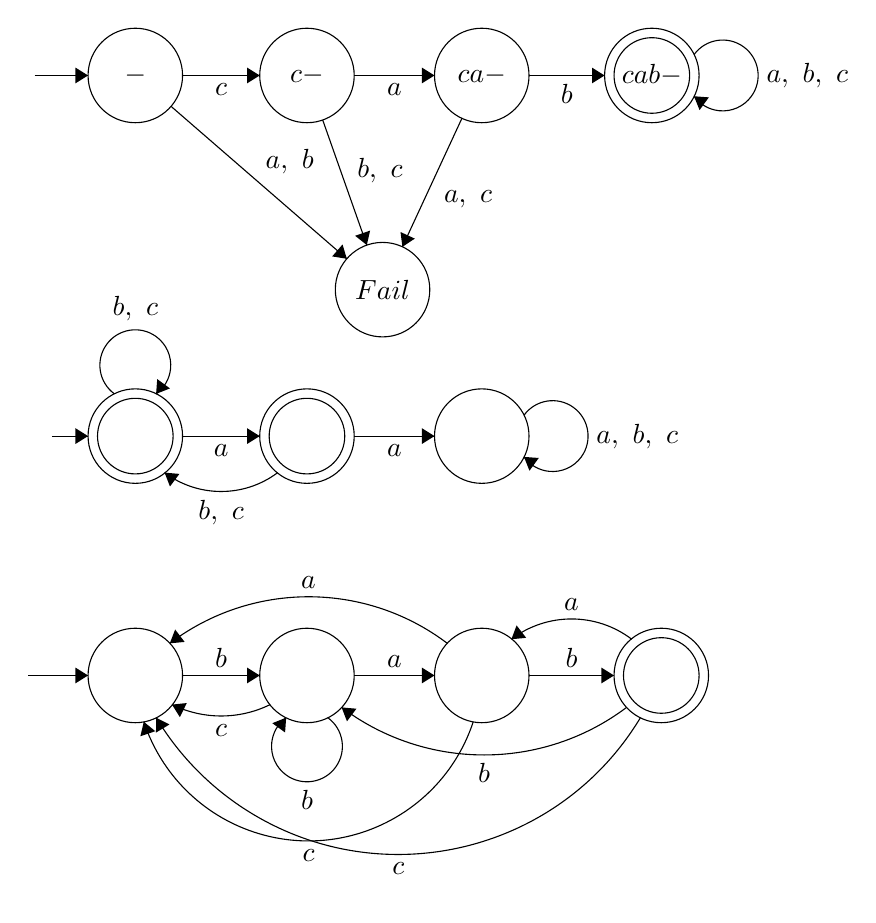
\begin{tikzpicture}[scale=0.2]
        \tikzstyle{every node}+=[inner sep=0pt]
        \draw [black] (8.2,-6.2) circle (3);
        \draw (8.2,-6.2) node {$-$};
        \draw [black] (19.1,-6.2) circle (3);
        \draw (19.1,-6.2) node {$c-$};
        \draw [black] (30.2,-6.2) circle (3);
        \draw (30.2,-6.2) node {$ca-$};
        \draw [black] (41,-6.2) circle (3);
        \draw (41,-6.2) node {$cab-$};
        \draw [black] (41,-6.2) circle (2.4);
        \draw [black] (23.9,-19.8) circle (3);
        \draw (23.9,-19.8) node {$Fail$};
        \draw [black] (8.2,-29.1) circle (3);
        \draw [black] (8.2,-29.1) circle (2.4);
        \draw [black] (19.1,-29.1) circle (3);
        \draw [black] (19.1,-29.1) circle (2.4);
        \draw [black] (30.2,-29.1) circle (3);
        \draw [black] (8.2,-44.3) circle (3);
        \draw [black] (19.1,-44.3) circle (3);
        \draw [black] (30.2,-44.3) circle (3);
        \draw [black] (41.6,-44.3) circle (3);
        \draw [black] (41.6,-44.3) circle (2.4);
        \draw [black] (11.2,-6.2) -- (16.1,-6.2);
        \fill [black] (16.1,-6.2) -- (15.3,-5.7) -- (15.3,-6.7);
        \draw (13.65,-6.7) node [below] {$c$};
        \draw [black] (22.1,-6.2) -- (27.2,-6.2);
        \fill [black] (27.2,-6.2) -- (26.4,-5.7) -- (26.4,-6.7);
        \draw (24.65,-6.7) node [below] {$a$};
        \draw [black] (33.2,-6.2) -- (38,-6.2);
        \fill [black] (38,-6.2) -- (37.2,-5.7) -- (37.2,-6.7);
        \draw (35.6,-6.7) node [below] {$b$};
        \draw [black] (43.68,-4.877) arc (144:-144:2.25);
        \draw (48.25,-6.2) node [right] {$a,\mbox{ }b,\mbox{ }c$};
        \fill [black] (43.68,-7.52) -- (44.03,-8.4) -- (44.62,-7.59);
        \draw [black] (1.8,-6.2) -- (5.2,-6.2);
        \fill [black] (5.2,-6.2) -- (4.4,-5.7) -- (4.4,-6.7);
        \draw [black] (10.47,-8.16) -- (21.63,-17.84);
        \fill [black] (21.63,-17.84) -- (21.36,-16.93) -- (20.7,-17.69);
        \draw (18,-12.51) node [above] {$a,\mbox{ }b$};
        \draw [black] (20.1,-9.03) -- (22.9,-16.97);
        \fill [black] (22.9,-16.97) -- (23.11,-16.05) -- (22.16,-16.38);
        \draw (22.26,-12.24) node [right] {$b,\mbox{ }c$};
        \draw [black] (28.94,-8.92) -- (25.16,-17.08);
        \fill [black] (25.16,-17.08) -- (25.95,-16.56) -- (25.04,-16.14);
        \draw (27.77,-14.03) node [right] {$a,\mbox{ }c$};
        \draw [black] (11.2,-29.1) -- (16.1,-29.1);
        \fill [black] (16.1,-29.1) -- (15.3,-28.6) -- (15.3,-29.6);
        \draw (13.65,-29.6) node [below] {$a$};
        \draw [black] (22.1,-29.1) -- (27.2,-29.1);
        \fill [black] (27.2,-29.1) -- (26.4,-28.6) -- (26.4,-29.6);
        \draw (24.65,-29.6) node [below] {$a$};
        \draw [black] (6.877,-26.42) arc (234:-54:2.25);
        \draw (8.2,-21.85) node [above] {$b,\mbox{ }c$};
        \fill [black] (9.52,-26.42) -- (10.4,-26.07) -- (9.59,-25.48);
        \draw [black] (2.9,-29.1) -- (5.2,-29.1);
        \fill [black] (5.2,-29.1) -- (4.4,-28.6) -- (4.4,-29.6);
        \draw [black] (32.88,-27.777) arc (144:-144:2.25);
        \draw (37.45,-29.1) node [right] {$a,\mbox{ }b,\mbox{ }c$};
        \fill [black] (32.88,-30.42) -- (33.23,-31.3) -- (33.82,-30.49);
        \draw [black] (17.244,-31.417) arc (-53.06845:-126.93155:5.981);
        \fill [black] (10.06,-31.42) -- (10.4,-32.3) -- (11,-31.5);
        \draw (13.65,-33.12) node [below] {$b,\mbox{ }c$};
        \draw [black] (1.4,-44.3) -- (5.2,-44.3);
        \fill [black] (5.2,-44.3) -- (4.4,-43.8) -- (4.4,-44.8);
        \draw [black] (11.2,-44.3) -- (16.1,-44.3);
        \fill [black] (16.1,-44.3) -- (15.3,-43.8) -- (15.3,-44.8);
        \draw (13.65,-43.8) node [above] {$b$};
        \draw [black] (33.2,-44.3) -- (38.6,-44.3);
        \fill [black] (38.6,-44.3) -- (37.8,-43.8) -- (37.8,-44.8);
        \draw (35.9,-43.8) node [above] {$b$};
        \draw [black] (22.1,-44.3) -- (27.2,-44.3);
        \fill [black] (27.2,-44.3) -- (26.4,-43.8) -- (26.4,-44.8);
        \draw (24.65,-43.8) node [above] {$a$};
        \draw [black] (32.079,-41.997) arc (127.19658:52.80342:6.321);
        \fill [black] (32.08,-42) -- (33.02,-41.91) -- (32.41,-41.12);
        \draw (35.9,-40.21) node [above] {$a$};
        \draw [black] (10.391,-42.258) arc (127.1047:52.8953:14.603);
        \fill [black] (10.39,-42.26) -- (11.33,-42.17) -- (10.73,-41.38);
        \draw (19.2,-38.8) node [above] {$a$};
        \draw [black] (20.423,-46.98) arc (54:-234:2.25);
        \draw (19.1,-51.55) node [below] {$b$};
        \fill [black] (17.78,-46.98) -- (16.9,-47.33) -- (17.71,-47.92);
        \draw [black] (39.396,-46.328) arc (-53.08319:-126.91681:15.061);
        \fill [black] (21.3,-46.33) -- (21.64,-47.21) -- (22.24,-46.41);
        \draw (30.35,-49.85) node [below] {$b$};
        \draw [black] (40.272,-46.986) arc (-31.10309:-148.89691:17.952);
        \fill [black] (9.53,-46.99) -- (9.51,-47.93) -- (10.37,-47.41);
        \draw (24.9,-56.16) node [below] {$c$};
        \draw [black] (29.658,-47.241) arc (-18.24627:-161.75373:11.012);
        \fill [black] (8.74,-47.24) -- (8.52,-48.16) -- (9.47,-47.84);
        \draw (19.2,-55.31) node [below] {$c$};
        \draw [black] (16.765,-46.148) arc (-63.81534:-116.18466:7.06);
        \fill [black] (10.53,-46.15) -- (11.03,-46.95) -- (11.47,-46.05);
        \draw (13.65,-47.37) node [below] {$c$};
        \end{tikzpicture}
        \end{center}

        \newpage

        \item The following NFA will check to see that there are only two characters present. As soon as a third is present in the string, there is nowhere to proceed and the machine fails. (The machine is presented in an unreduced form to make it easier to understand at a glance without having to decipher criss crossed lines. The accepting states labeled with the same letters could be combined into 1 state each.)
        \begin{center}
        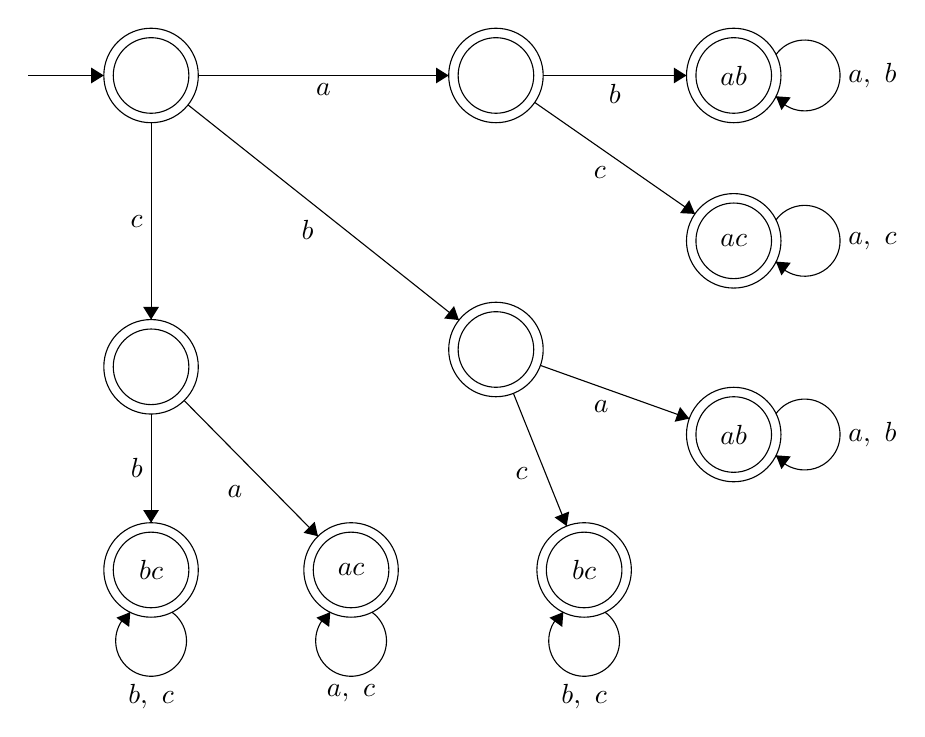
\begin{tikzpicture}[scale=0.2]
        \tikzstyle{every node}+=[inner sep=0pt]
        \draw [black] (11.6,-9.1) circle (3);
        \draw [black] (11.6,-9.1) circle (2.4);
        \draw [black] (33.5,-9.1) circle (3);
        \draw [black] (33.5,-9.1) circle (2.4);
        \draw [black] (33.5,-26.5) circle (3);
        \draw [black] (33.5,-26.5) circle (2.4);
        \draw [black] (11.6,-27.6) circle (3);
        \draw [black] (11.6,-27.6) circle (2.4);
        \draw [black] (48.6,-9.1) circle (3);
        \draw (48.6,-9.1) node {$ab$};
        \draw [black] (48.6,-9.1) circle (2.4);
        \draw [black] (48.6,-19.6) circle (3);
        \draw (48.6,-19.6) node {$ac$};
        \draw [black] (48.6,-19.6) circle (2.4);
        \draw [black] (48.6,-31.9) circle (3);
        \draw (48.6,-31.9) node {$ab$};
        \draw [black] (48.6,-31.9) circle (2.4);
        \draw [black] (39.1,-40.5) circle (3);
        \draw (39.1,-40.5) node {$bc$};
        \draw [black] (39.1,-40.5) circle (2.4);
        \draw [black] (24.3,-40.5) circle (3);
        \draw (24.3,-40.5) node {$ac$};
        \draw [black] (24.3,-40.5) circle (2.4);
        \draw [black] (11.6,-40.5) circle (3);
        \draw (11.6,-40.5) node {$bc$};
        \draw [black] (11.6,-40.5) circle (2.4);
        \draw [black] (3.8,-9.1) -- (8.6,-9.1);
        \fill [black] (8.6,-9.1) -- (7.8,-8.6) -- (7.8,-9.6);
        \draw [black] (13.95,-10.97) -- (31.15,-24.63);
        \fill [black] (31.15,-24.63) -- (30.84,-23.74) -- (30.21,-24.53);
        \draw (21.54,-18.29) node [below] {$b$};
        \draw [black] (14.6,-9.1) -- (30.5,-9.1);
        \fill [black] (30.5,-9.1) -- (29.7,-8.6) -- (29.7,-9.6);
        \draw (22.55,-9.6) node [below] {$a$};
        \draw [black] (11.6,-12.1) -- (11.6,-24.6);
        \fill [black] (11.6,-24.6) -- (12.1,-23.8) -- (11.1,-23.8);
        \draw (11.1,-18.35) node [left] {$c$};
        \draw [black] (34.61,-29.29) -- (37.99,-37.71);
        \fill [black] (37.99,-37.71) -- (38.15,-36.79) -- (37.22,-37.16);
        \draw (35.55,-34.38) node [left] {$c$};
        \draw [black] (36.32,-27.51) -- (45.78,-30.89);
        \fill [black] (45.78,-30.89) -- (45.19,-30.15) -- (44.85,-31.09);
        \draw (40.18,-29.73) node [below] {$a$};
        \draw [black] (36.5,-9.1) -- (45.6,-9.1);
        \fill [black] (45.6,-9.1) -- (44.8,-8.6) -- (44.8,-9.6);
        \draw (41.05,-9.6) node [below] {$b$};
        \draw [black] (35.96,-10.81) -- (46.14,-17.89);
        \fill [black] (46.14,-17.89) -- (45.77,-17.02) -- (45.19,-17.84);
        \draw (40.1,-14.85) node [below] {$c$};
        \draw [black] (51.28,-7.777) arc (144:-144:2.25);
        \draw (55.85,-9.1) node [right] {$a,\mbox{ }b$};
        \fill [black] (51.28,-10.42) -- (51.63,-11.3) -- (52.22,-10.49);
        \draw [black] (51.28,-18.277) arc (144:-144:2.25);
        \draw (55.85,-19.6) node [right] {$a,\mbox{ }c$};
        \fill [black] (51.28,-20.92) -- (51.63,-21.8) -- (52.22,-20.99);
        \draw [black] (51.28,-30.577) arc (144:-144:2.25);
        \draw (55.85,-31.9) node [right] {$a,\mbox{ }b$};
        \fill [black] (51.28,-33.22) -- (51.63,-34.1) -- (52.22,-33.29);
        \draw [black] (40.423,-43.18) arc (54:-234:2.25);
        \draw (39.1,-47.75) node [below] {$b,\mbox{ }c$};
        \fill [black] (37.78,-43.18) -- (36.9,-43.53) -- (37.71,-44.12);
        \draw [black] (13.7,-29.74) -- (22.2,-38.36);
        \fill [black] (22.2,-38.36) -- (21.99,-37.44) -- (21.28,-38.14);
        \draw (17.42,-35.52) node [left] {$a$};
        \draw [black] (25.623,-43.18) arc (54:-234:2.25);
        \draw (24.3,-47.75) node [below] {$a,\mbox{ }c$};
        \fill [black] (22.98,-43.18) -- (22.1,-43.53) -- (22.91,-44.12);
        \draw [black] (11.6,-30.6) -- (11.6,-37.5);
        \fill [black] (11.6,-37.5) -- (12.1,-36.7) -- (11.1,-36.7);
        \draw (11.1,-34.05) node [left] {$b$};
        \draw [black] (12.923,-43.18) arc (54:-234:2.25);
        \draw (11.6,-47.75) node [below] {$b,\mbox{ }c$};
        \fill [black] (10.28,-43.18) -- (9.4,-43.53) -- (10.21,-44.12);
        \end{tikzpicture}
        \end{center}

        \newpage

        \item This NFA can be produced using careful product construction of two NFAs: one that tracks the third to last bit (top) and one that tracks the third bit (bottom). Let the top NFA be $M$ and the bottom NFA be $N$. The accepting states of $M\times N$ is given as $F = \{m_an_a, m_bn_b\}$ indicating that the 3rd first and 3rd last bits are the same.
        \begin{center}
        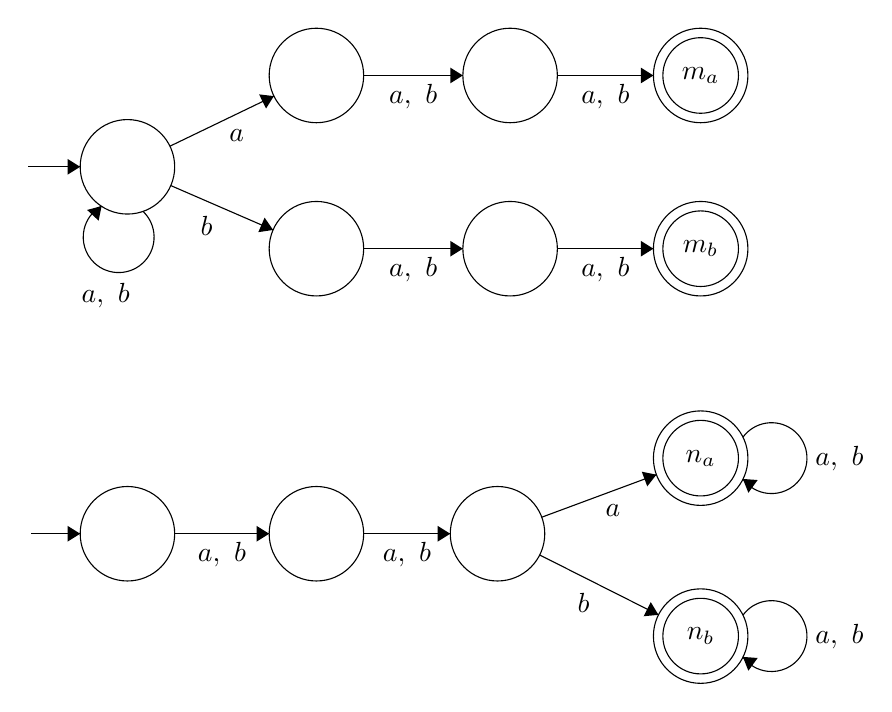
\begin{tikzpicture}[scale=0.2]
        \tikzstyle{every node}+=[inner sep=0pt]
        \draw [black] (8.6,-14.3) circle (3);
        \draw [black] (20.6,-8.5) circle (3);
        \draw [black] (20.6,-19.5) circle (3);
        \draw [black] (32.9,-8.5) circle (3);
        \draw [black] (32.9,-19.5) circle (3);
        \draw [black] (45,-8.5) circle (3);
        \draw (45,-8.5) node {$m_a$};
        \draw [black] (45,-8.5) circle (2.4);
        \draw [black] (45,-19.5) circle (3);
        \draw (45,-19.5) node {$m_b$};
        \draw [black] (45,-19.5) circle (2.4);
        \draw [black] (8.6,-37.6) circle (3);
        \draw [black] (20.6,-37.6) circle (3);
        \draw [black] (32.1,-37.6) circle (3);
        \draw [black] (45,-32.8) circle (3);
        \draw (45,-32.8) node {$n_a$};
        \draw [black] (45,-32.8) circle (2.4);
        \draw [black] (45,-44.1) circle (3);
        \draw (45,-44.1) node {$n_b$};
        \draw [black] (45,-44.1) circle (2.4);
        \draw [black] (35.9,-8.5) -- (42,-8.5);
        \fill [black] (42,-8.5) -- (41.2,-8) -- (41.2,-9);
        \draw (38.95,-9) node [below] {$a,\mbox{ }b$};
        \draw [black] (35.9,-19.5) -- (42,-19.5);
        \fill [black] (42,-19.5) -- (41.2,-19) -- (41.2,-20);
        \draw (38.95,-20) node [below] {$a,\mbox{ }b$};
        \draw [black] (23.6,-19.5) -- (29.9,-19.5);
        \fill [black] (29.9,-19.5) -- (29.1,-19) -- (29.1,-20);
        \draw (26.75,-20) node [below] {$a,\mbox{ }b$};
        \draw [black] (23.6,-8.5) -- (29.9,-8.5);
        \fill [black] (29.9,-8.5) -- (29.1,-8) -- (29.1,-9);
        \draw (26.75,-9) node [below] {$a,\mbox{ }b$};
        \draw [black] (11.3,-12.99) -- (17.9,-9.81);
        \fill [black] (17.9,-9.81) -- (16.96,-9.7) -- (17.4,-10.6);
        \draw (15.53,-11.91) node [below] {$a$};
        \draw [black] (11.35,-15.49) -- (17.85,-18.31);
        \fill [black] (17.85,-18.31) -- (17.31,-17.53) -- (16.91,-18.45);
        \draw (13.63,-17.41) node [below] {$b$};
        \draw [black] (2.3,-14.3) -- (5.6,-14.3);
        \fill [black] (5.6,-14.3) -- (4.8,-13.8) -- (4.8,-14.8);
        \draw [black] (11.6,-37.6) -- (17.6,-37.6);
        \fill [black] (17.6,-37.6) -- (16.8,-37.1) -- (16.8,-38.1);
        \draw (14.6,-38.1) node [below] {$a,\mbox{ }b$};
        \draw [black] (23.6,-37.6) -- (29.1,-37.6);
        \fill [black] (29.1,-37.6) -- (28.3,-37.1) -- (28.3,-38.1);
        \draw (26.35,-38.1) node [below] {$a,\mbox{ }b$};
        \draw [black] (34.91,-36.55) -- (42.19,-33.85);
        \fill [black] (42.19,-33.85) -- (41.26,-33.66) -- (41.61,-34.59);
        \draw (39.43,-35.72) node [below] {$a$};
        \draw [black] (34.78,-38.95) -- (42.32,-42.75);
        \fill [black] (42.32,-42.75) -- (41.83,-41.94) -- (41.38,-42.84);
        \draw (37.56,-41.35) node [below] {$b$};
        \draw [black] (2.5,-37.6) -- (5.6,-37.6);
        \fill [black] (5.6,-37.6) -- (4.8,-37.1) -- (4.8,-38.1);
        \draw [black] (47.68,-31.477) arc (144:-144:2.25);
        \draw (52.25,-32.8) node [right] {$a,\mbox{ }b$};
        \fill [black] (47.68,-34.12) -- (48.03,-35) -- (48.62,-34.19);
        \draw [black] (47.68,-42.777) arc (144:-144:2.25);
        \draw (52.25,-44.1) node [right] {$a,\mbox{ }b$};
        \fill [black] (47.68,-45.42) -- (48.03,-46.3) -- (48.62,-45.49);
        \draw [black] (9.58,-17.123) arc (46.87498:-241.12502:2.25);
        \draw (7.22,-21.67) node [below] {$a,\mbox{ }b$};
        \fill [black] (6.96,-16.79) -- (6.04,-17.04) -- (6.77,-17.72);
        \end{tikzpicture}
        \end{center}

        \newpage

        \item This NFA is created through applciation of closure properties on the sub NFAs below. First let us label them from top to bottom as $B_0, B_1, P_0, $ and $P_1$ respectively. They represent the third to last bit being 0, the third from last bit being 1, the parity being 0, and the parity being 1 respectively as well. The NFA combining all of these features is given as $(P_0 \cap B_0)\cup(P_1 \cap B_1)$.
        \begin{center}
        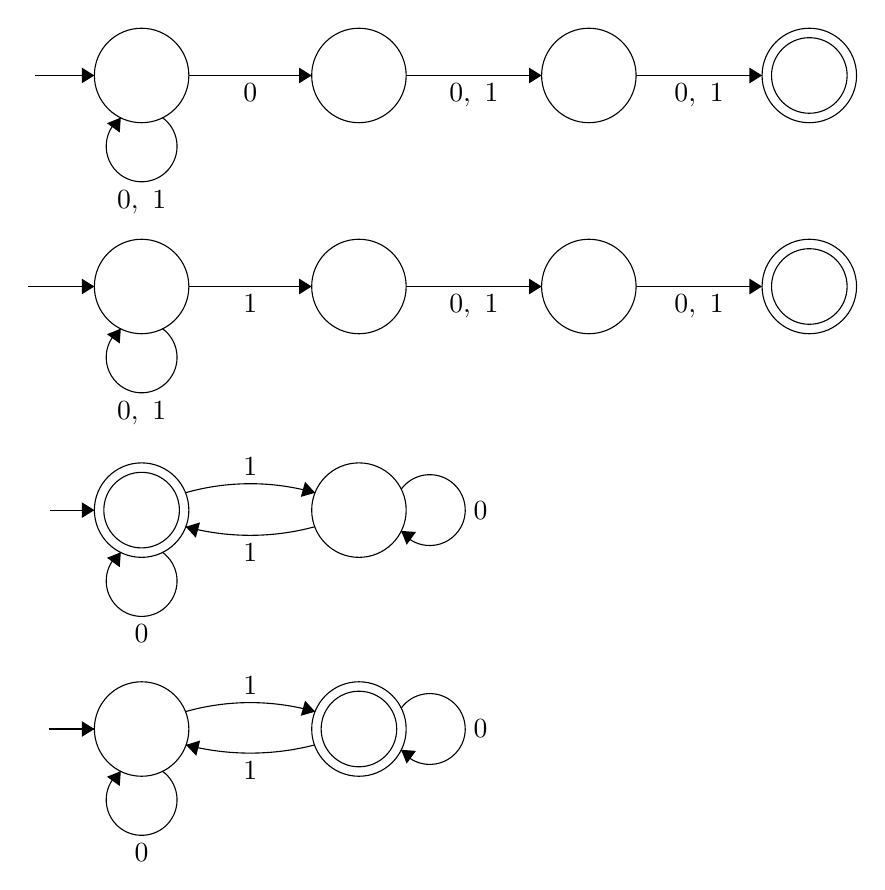
\begin{tikzpicture}[scale=0.2]
        \tikzstyle{every node}+=[inner sep=0pt]
        \draw [black] (8.5,-7.7) circle (3);
        \draw [black] (22.3,-7.7) circle (3);
        \draw [black] (36.9,-7.7) circle (3);
        \draw [black] (50.9,-7.7) circle (3);
        \draw [black] (50.9,-7.7) circle (2.4);
        \draw [black] (8.5,-21.1) circle (3);
        \draw [black] (22.3,-21.1) circle (3);
        \draw [black] (36.9,-21.1) circle (3);
        \draw [black] (50.9,-21.1) circle (3);
        \draw [black] (50.9,-21.1) circle (2.4);
        \draw [black] (8.5,-35.3) circle (3);
        \draw [black] (8.5,-35.3) circle (2.4);
        \draw [black] (22.3,-35.3) circle (3);
        \draw [black] (8.5,-49.2) circle (3);
        \draw [black] (22.3,-49.2) circle (3);
        \draw [black] (22.3,-49.2) circle (2.4);
        \draw [black] (11.285,-48.097) arc (105.88718:74.11282:15.034);
        \fill [black] (19.52,-48.1) -- (18.88,-47.4) -- (18.61,-48.36);
        \draw (15.4,-47.02) node [above] {$1$};
        \draw [black] (19.48,-50.212) arc (-75.51855:-104.48145:16.317);
        \fill [black] (11.32,-50.21) -- (11.97,-50.9) -- (12.22,-49.93);
        \draw (15.4,-51.23) node [below] {$1$};
        \draw [black] (24.98,-47.877) arc (144:-144:2.25);
        \draw (29.55,-49.2) node [right] {$0$};
        \fill [black] (24.98,-50.52) -- (25.33,-51.4) -- (25.92,-50.59);
        \draw [black] (9.823,-51.88) arc (54:-234:2.25);
        \draw (8.5,-56.45) node [below] {$0$};
        \fill [black] (7.18,-51.88) -- (6.3,-52.23) -- (7.11,-52.82);
        \draw [black] (2.6,-49.2) -- (5.5,-49.2);
        \fill [black] (5.5,-49.2) -- (4.7,-48.7) -- (4.7,-49.7);
        \draw [black] (2.7,-35.3) -- (5.5,-35.3);
        \fill [black] (5.5,-35.3) -- (4.7,-34.8) -- (4.7,-35.8);
        \draw [black] (9.823,-37.98) arc (54:-234:2.25);
        \draw (8.5,-42.55) node [below] {$0$};
        \fill [black] (7.18,-37.98) -- (6.3,-38.33) -- (7.11,-38.92);
        \draw [black] (11.285,-34.197) arc (105.88718:74.11282:15.034);
        \fill [black] (19.52,-34.2) -- (18.88,-33.5) -- (18.61,-34.46);
        \draw (15.4,-33.12) node [above] {$1$};
        \draw [black] (19.497,-36.356) arc (-74.84075:-105.15925:15.667);
        \fill [black] (11.3,-36.36) -- (11.94,-37.05) -- (12.21,-36.08);
        \draw (15.4,-37.4) node [below] {$1$};
        \draw [black] (24.98,-33.977) arc (144:-144:2.25);
        \draw (29.55,-35.3) node [right] {$0$};
        \fill [black] (24.98,-36.62) -- (25.33,-37.5) -- (25.92,-36.69);
        \draw [black] (9.823,-10.38) arc (54:-234:2.25);
        \draw (8.5,-14.95) node [below] {$0,\mbox{ }1$};
        \fill [black] (7.18,-10.38) -- (6.3,-10.73) -- (7.11,-11.32);
        \draw [black] (1.7,-7.7) -- (5.5,-7.7);
        \fill [black] (5.5,-7.7) -- (4.7,-7.2) -- (4.7,-8.2);
        \draw [black] (1.3,-21.1) -- (5.5,-21.1);
        \fill [black] (5.5,-21.1) -- (4.7,-20.6) -- (4.7,-21.6);
        \draw [black] (9.823,-23.78) arc (54:-234:2.25);
        \draw (8.5,-28.35) node [below] {$0,\mbox{ }1$};
        \fill [black] (7.18,-23.78) -- (6.3,-24.13) -- (7.11,-24.72);
        \draw [black] (11.5,-21.1) -- (19.3,-21.1);
        \fill [black] (19.3,-21.1) -- (18.5,-20.6) -- (18.5,-21.6);
        \draw (15.4,-21.6) node [below] {$1$};
        \draw [black] (11.5,-7.7) -- (19.3,-7.7);
        \fill [black] (19.3,-7.7) -- (18.5,-7.2) -- (18.5,-8.2);
        \draw (15.4,-8.2) node [below] {$0$};
        \draw [black] (25.3,-7.7) -- (33.9,-7.7);
        \fill [black] (33.9,-7.7) -- (33.1,-7.2) -- (33.1,-8.2);
        \draw (29.6,-8.2) node [below] {$0,\mbox{ }1$};
        \draw [black] (25.3,-21.1) -- (33.9,-21.1);
        \fill [black] (33.9,-21.1) -- (33.1,-20.6) -- (33.1,-21.6);
        \draw (29.6,-21.6) node [below] {$0,\mbox{ }1$};
        \draw [black] (39.9,-7.7) -- (47.9,-7.7);
        \fill [black] (47.9,-7.7) -- (47.1,-7.2) -- (47.1,-8.2);
        \draw (43.9,-8.2) node [below] {$0,\mbox{ }1$};
        \draw [black] (39.9,-21.1) -- (47.9,-21.1);
        \fill [black] (47.9,-21.1) -- (47.1,-20.6) -- (47.1,-21.6);
        \draw (43.9,-21.6) node [below] {$0,\mbox{ }1$};
        \end{tikzpicture}
        \end{center}
    \end{enumerate}
    \item Let $L_A$ be the language accepted by $A$ where $L_A = \{x \in \{a, b\}^*| 'b' \in x \}$. Let $L_B$ be the language accepted by $B$ where $L_B = \{x \in \{a, b\}^*| 'b' \notin x \}$. They can be seen below:

    % Put the DFAs in here.
    \begin{center}
    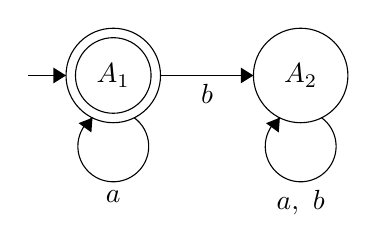
\begin{tikzpicture}[scale=0.2]
    \tikzstyle{every node}+=[inner sep=0pt]
    \draw [black] (8.3,-6.5) circle (3);
    \draw (8.3,-6.5) node {$A_1$};
    \draw [black] (8.3,-6.5) circle (2.4);
    \draw [black] (20.2,-6.5) circle (3);
    \draw (20.2,-6.5) node {$A_2$};
    \draw [black] (2.9,-6.5) -- (5.3,-6.5);
    \fill [black] (5.3,-6.5) -- (4.5,-6) -- (4.5,-7);
    \draw [black] (11.3,-6.5) -- (17.2,-6.5);
    \fill [black] (17.2,-6.5) -- (16.4,-6) -- (16.4,-7);
    \draw (14.25,-7) node [below] {$b$};
    \draw [black] (21.523,-9.18) arc (54:-234:2.25);
    \draw (20.2,-13.75) node [below] {$a,\mbox{ }b$};
    \fill [black] (18.88,-9.18) -- (18,-9.53) -- (18.81,-10.12);
    \draw [black] (9.623,-9.18) arc (54:-234:2.25);
    \draw (8.3,-13.75) node [below] {$a$};
    \fill [black] (6.98,-9.18) -- (6.1,-9.53) -- (6.91,-10.12);
    \end{tikzpicture}
    \end{center}
    \begin{center}
    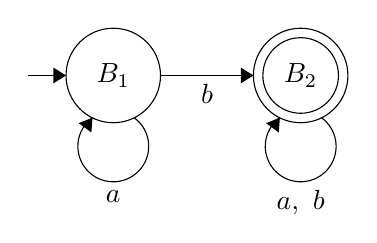
\begin{tikzpicture}[scale=0.2]
    \tikzstyle{every node}+=[inner sep=0pt]
    \draw [black] (8.3,-6.5) circle (3);
    \draw (8.3,-6.5) node {$B_1$};
    \draw [black] (20.2,-6.5) circle (3);
    \draw (20.2,-6.5) node {$B_2$};
    \draw [black] (20.2,-6.5) circle (2.4);
    \draw [black] (2.9,-6.5) -- (5.3,-6.5);
    \fill [black] (5.3,-6.5) -- (4.5,-6) -- (4.5,-7);
    \draw [black] (11.3,-6.5) -- (17.2,-6.5);
    \fill [black] (17.2,-6.5) -- (16.4,-6) -- (16.4,-7);
    \draw (14.25,-7) node [below] {$b$};
    \draw [black] (21.523,-9.18) arc (54:-234:2.25);
    \draw (20.2,-13.75) node [below] {$a,\mbox{ }b$};
    \fill [black] (18.88,-9.18) -- (18,-9.53) -- (18.81,-10.12);
    \draw [black] (9.623,-9.18) arc (54:-234:2.25);
    \draw (8.3,-13.75) node [below] {$a$};
    \fill [black] (6.98,-9.18) -- (6.1,-9.53) -- (6.91,-10.12);
    \end{tikzpicture}
    \end{center}

    Next, let $L_{A \times B}$ be the language accepted by a DFA that is created with product construction from $A \cup B$. This DFA looks like this and accepts $\{x \in \{a, b\}^*|'b'\in x$ or $'b' \notin x\}$. On the left is the direct product construction DFA, and on the right is the same DFA with unreachable states removed.

    % Put the product DFA in here.
    \begin{center}
    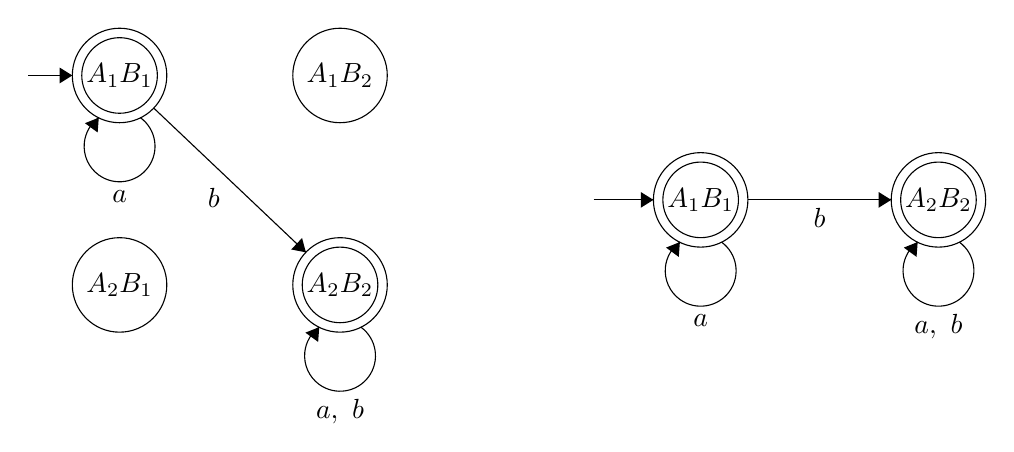
\begin{tikzpicture}[scale=0.2]
    \tikzstyle{every node}+=[inner sep=0pt]
    \draw [black] (8.5,-7) circle (3);
    \draw (8.5,-7) node {$A_1B_1$};
    \draw [black] (8.5,-7) circle (2.4);
    \draw [black] (22.5,-7) circle (3);
    \draw (22.5,-7) node {$A_1B_2$};
    \draw [black] (8.5,-20.3) circle (3);
    \draw (8.5,-20.3) node {$A_2B_1$};
    \draw [black] (22.5,-20.3) circle (3);
    \draw (22.5,-20.3) node {$A_2B_2$};
    \draw [black] (22.5,-20.3) circle (2.4);
    \draw [black] (45.4,-14.9) circle (3);
    \draw (45.4,-14.9) node {$A_1B_1$};
    \draw [black] (45.4,-14.9) circle (2.4);
    \draw [black] (60.5,-14.9) circle (3);
    \draw (60.5,-14.9) node {$A_2B_2$};
    \draw [black] (60.5,-14.9) circle (2.4);
    \draw [black] (10.67,-9.07) -- (20.33,-18.23);
    \fill [black] (20.33,-18.23) -- (20.09,-17.32) -- (19.4,-18.05);
    \draw (14.48,-14.13) node [below] {$b$};
    \draw [black] (2.7,-7) -- (5.5,-7);
    \fill [black] (5.5,-7) -- (4.7,-6.5) -- (4.7,-7.5);
    \draw [black] (9.823,-9.68) arc (54:-234:2.25);
    \draw (8.5,-14.25) node [below] {$a$};
    \fill [black] (7.18,-9.68) -- (6.3,-10.03) -- (7.11,-10.62);
    \draw [black] (23.823,-22.98) arc (54:-234:2.25);
    \draw (22.5,-27.55) node [below] {$a,\mbox{ }b$};
    \fill [black] (21.18,-22.98) -- (20.3,-23.33) -- (21.11,-23.92);
    \draw [black] (38.6,-14.9) -- (42.4,-14.9);
    \fill [black] (42.4,-14.9) -- (41.6,-14.4) -- (41.6,-15.4);
    \draw [black] (48.4,-14.9) -- (57.5,-14.9);
    \fill [black] (57.5,-14.9) -- (56.7,-14.4) -- (56.7,-15.4);
    \draw (52.95,-15.4) node [below] {$b$};
    \draw [black] (46.723,-17.58) arc (54:-234:2.25);
    \draw (45.4,-22.15) node [below] {$a$};
    \fill [black] (44.08,-17.58) -- (43.2,-17.93) -- (44.01,-18.52);
    \draw [black] (61.823,-17.58) arc (54:-234:2.25);
    \draw (60.5,-22.15) node [below] {$a,\mbox{ }b$};
    \fill [black] (59.18,-17.58) -- (58.3,-17.93) -- (59.11,-18.52);
    \end{tikzpicture}
    \end{center}

    This DFA is not a minimal DFA as demonstrated by the below DFA. It accepts all of the same strings and has only 1 state as opposed to 2 states.

    % Put the final DFA here
    \begin{center}
    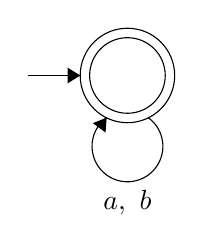
\begin{tikzpicture}[scale=0.2]
    \tikzstyle{every node}+=[inner sep=0pt]
    \draw [black] (10.6,-8) circle (3);
    \draw [black] (10.6,-8) circle (2.4);
    \draw [black] (4.3,-8) -- (7.6,-8);
    \fill [black] (7.6,-8) -- (6.8,-7.5) -- (6.8,-8.5);
    \draw [black] (11.923,-10.68) arc (54:-234:2.25);
    \draw (10.6,-15.25) node [below] {$a,\mbox{ }b$};
    \fill [black] (9.28,-10.68) -- (8.4,-11.03) -- (9.21,-11.62);
    \end{tikzpicture}
    \end{center}

    \item Suppose $D$ is regular. Let $p$ be the pumping constant for $D$. Let $w = 0^p1^{2p}$. Then $w$ can be broken up into substrings $xyz$ where $|xy| \leq p$ and $0 \leq |y|$ such that $xy^iz$ exists for all $i$. \\

    Then we know that $x = 0^k, y = 0^l,$ and $z=0^{p-k-l}1^{2p}$ where $k \geq 0, l > 0$. \\

    Let $i = 2$. Then:
    \begin{align*}
        xy^2z &= 0^k0^{2l}0^{p-k-l}1^{2p} \\
        &= 0^{p+l}1^{2p} \in D
    \end{align*}

    But since $l \geq 0, p+l \neq p$ Thus, there are more 0s than $D$ is able to accept. Since this is a contradiction to our assumption that $D$ is regular, we know that it must be nonregular.
\end{enumerate}

\end{document}
